\documentclass[journal,onecolumn]{IEEEtran}

% correct bad hyphenation here
\hyphenation{op-tical net-works semi-conduc-tor}

\usepackage{cite}
\usepackage{amsmath,amssymb,amsfonts}
\usepackage{algorithmic}
\usepackage{graphicx}
\usepackage{textcomp}
\usepackage{xcolor}
\usepackage[brazilian]{babel}
\usepackage[utf8]{inputenc}
\usepackage[T1]{fontenc}
\usepackage{listings}
\usepackage{listings-golang}
\usepackage{color}
\usepackage{float}
\usepackage{multirow}
\usepackage{hyperref}

\definecolor{dkgreen}{rgb}{0,0.6,0}
\definecolor{gray}{rgb}{0.5,0.5,0.5}
\definecolor{mauve}{rgb}{0.58,0,0.82}

\lstset{frame=tb,
  language=Golang,
  aboveskip=3mm,
  belowskip=3mm,
  showstringspaces=false,
  columns=flexible,
  basicstyle={\small\ttfamily},
  numbers=none,
  numberstyle=\tiny\color{gray},
  keywordstyle=\color{blue},
  commentstyle=\color{dkgreen},
  stringstyle=\color{mauve},
  breaklines=true,
  breakatwhitespace=true,
  tabsize=3
}
\lstset{language=Golang}
\def\BibTeX{{\rm B\kern-.05em{\sc i\kern-.025em b}\kern-.08em
    T\kern-.1667em\lower.7ex\hbox{E}\kern-.125emX}}


\begin{document}

\title{Relatório da Atividade 4: Raft}

\author{\IEEEauthorblockN{Isabelle Ferreira de Oliveira}
\IEEEauthorblockA{\textit{CES-27 - Engenharia da Computação 2020} \\
\textit{Instituto Tecnológico de Aeronáutica (ITA)}\\
São José dos Campos, Brasil \\
isabelle.ferreira3000@gmail.com}
}

\maketitle

\begin{abstract}
Esse relatório documenta um trabalho com o protocolo Raft para consenso distribuído. Não será trabalhado com \textit{log replication}.
\end{abstract}

\begin{IEEEkeywords}
Raft, Golang, sistema distribuído
\end{IEEEkeywords}

\section{Implementação}

\subsection{Ao receber um AppendEntry (heartbeat)}
Subsection text here.

\subsubsection{Follower}
\subsubsection{Candidate}
\subsubsection{Leader}

\subsection{Ao receber um RequestVote}
Subsubsection text here.

\subsubsection{Follower}
\subsubsection{Candidate}
\subsubsection{Leader}

\subsection{Ao receber um Reply}
Subsubsection text here.

\subsubsection{Follower}
\subsubsection{Candidate}
\subsubsection{Leader}

\section{Resultados e Conclusões}

Na Figura \ref{funcionamento_normal}, foi apresentado uma captura de tela de um funcionamento com todas instâncias funcionando.

\begin{itemize}
\item Server 2 vira \textit{cadidate}
\item Server 2 recebe voto de 1
\item Server 3 vira \textit{candidate}
\item Server 1 nega voto para 3 (já votou em 2)
\item Server 2 nega voto para 3 (já é candidate)
\item Server 2 recebe voto de 4 e 5 (e vira leader)
\item Server 3 não consegue maioria dos votos
\item Server 3 faz \textit{Step Down}
\item Server 1, 3, 4 e 5 continuam como \textit{follower} indefinidamente, pois 2 é \textit{leader}

\end{itemize}

\begin{figure}[H]
\centering
\centerline{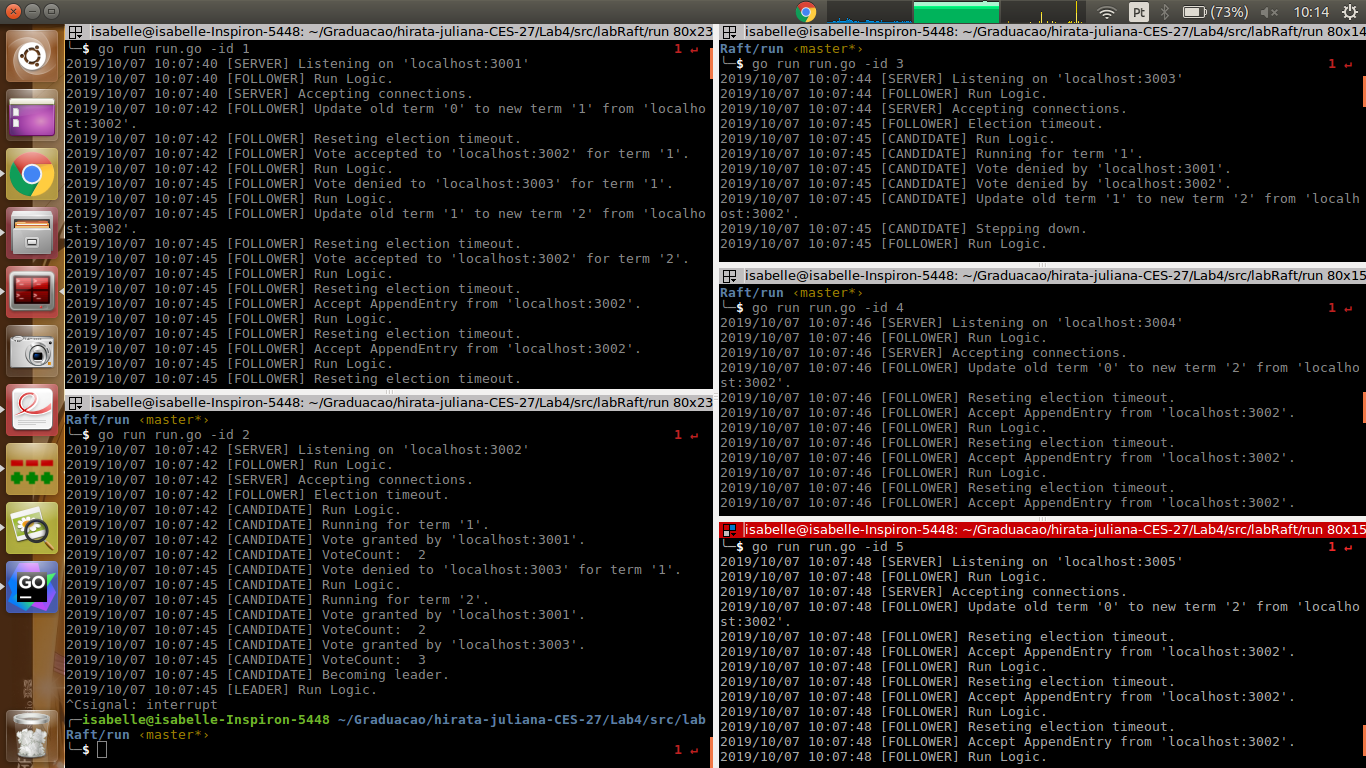
\includegraphics[scale=0.4]{imagens/funcionamento_normal.png}}
\caption{Funcionamento normal para os 5 processos.}
\label{funcionamento_normal}
\end{figure}

Na Figura \ref{falha_no_lider}, foi apresentado uma captura de tela de um funcionamento com falha do \textit{leader} (com outra instância assumindo a liderança) e retomada do servidor falho (com ele reconhecendo a liderança do outro).

\begin{itemize}
\item Server 3 (\textit{leader}) falha
\item Server 2 vira \textit{candidate}
\item Server 2 recebe voto de 1 e 5 (e vira \textit{leader}), e de 4
\item Server 3 é retomado e recebe \textit{AppendEntry} de 2 (que é o novo \textit{leader})
\item Server 1, 3, 4 e 5 continuam como \textit{follower} indefinidamente, pois 2 é \textit{leader}
\end{itemize}

\begin{figure}[H]
\centering
\centerline{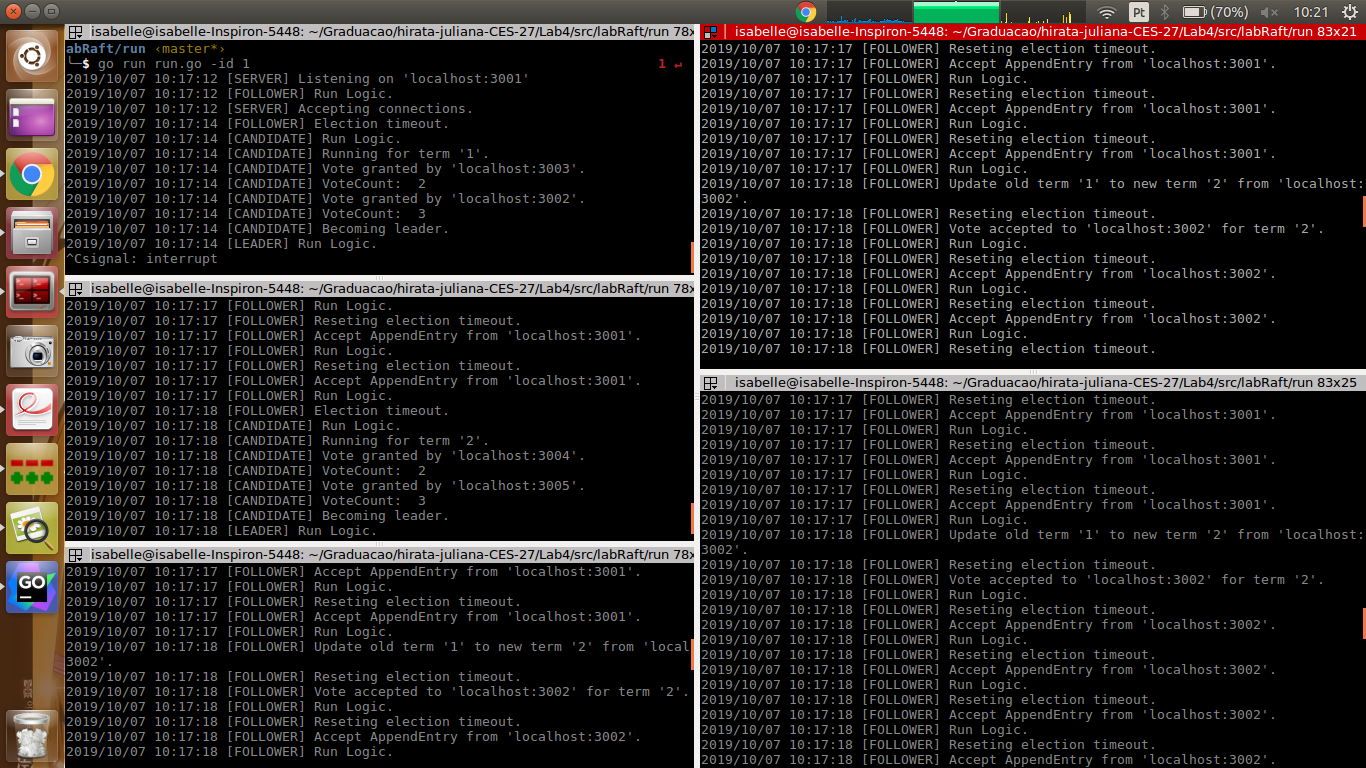
\includegraphics[scale=0.4]{imagens/falha_no_lider.png}}
\caption{Funcionamento após a falha no \textit{leader}, seguido de retomada do processo.}.
\label{falha_no_lider}
\end{figure}

Na Figura \ref{1_falha}, foi apresentado uma captura de tela de um funcionamento com falha de uma instância (o \textit{leader}), agora sem retomada do servidor falho. Note que outro servidor assume a liderança.

\begin{itemize}
\item Server 1 (leader) falha
\item Server 3 vira \textit{candidate}
\item Server 3 recebe voto de 4 e 2 (e vira \textit{leader}), e de 3 e 5
\item Server 2, 4 e 5 continuam como \textit{follower}, pois 3 é \textit{leader}
\end{itemize}

\begin{figure}[H]
\centering
\centerline{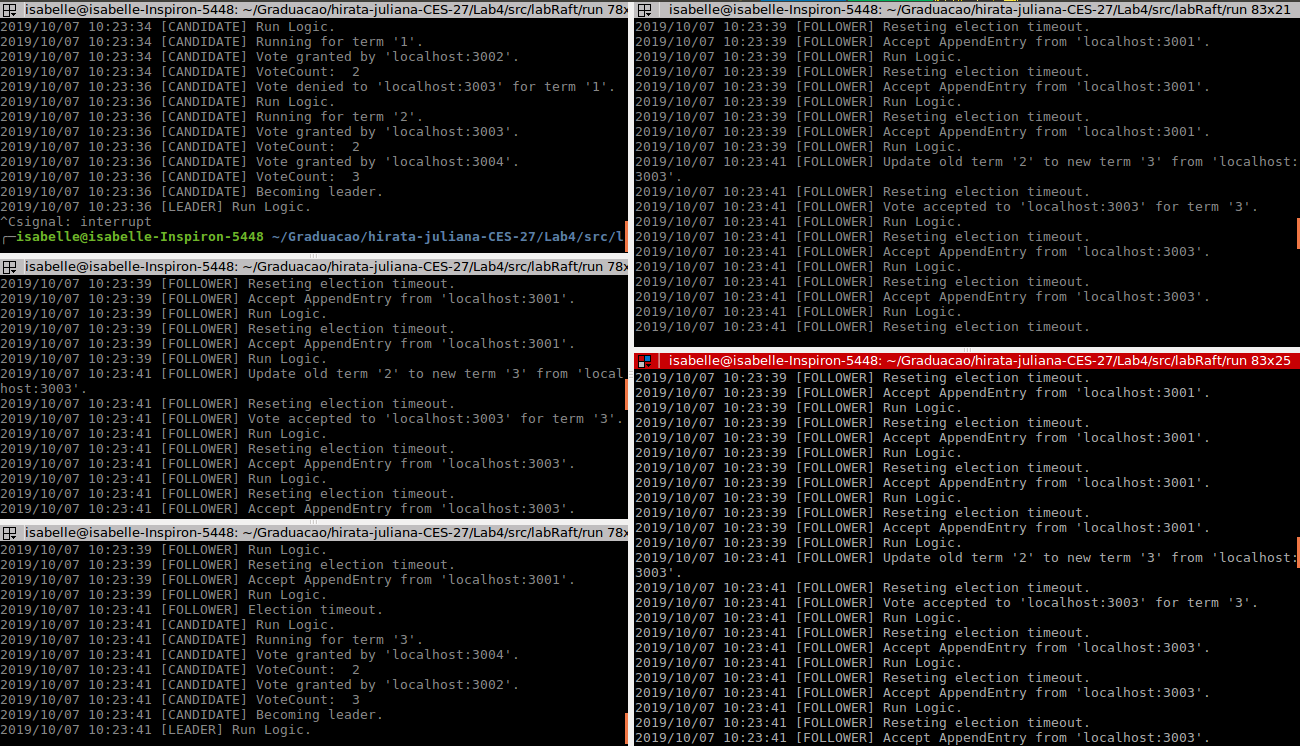
\includegraphics[scale=0.4]{imagens/1_falha.png}}
\caption{Funcionamento após a falha no \textit{leader}.}.
\label{1_falha}
\end{figure}

Na Figura \ref{2_falhas}, foi apresentado uma captura de tela de um funcionamento com falha de duas instâncias, também sem retomadas dos servidores falhos. Note que outro servidor assume a liderança.

\begin{itemize}
\item Server 1 (\textit{leader}) falha
\item Server 3 vira \textit{candidate}
\item Server 3 recebe voto de 4 e 2 (e vira \textit{leader})
\item Server 3 (\textit{leader}) falha
\item Server 4 vira \textit{candidate}
\item Server 4 recebe voto de 2 e 5 (e vira \textit{leader})
\item Server 5 continua como \textit{follower}, pois 4 é \textit{leader}
\end{itemize}

\begin{figure}[H]
\centering
\centerline{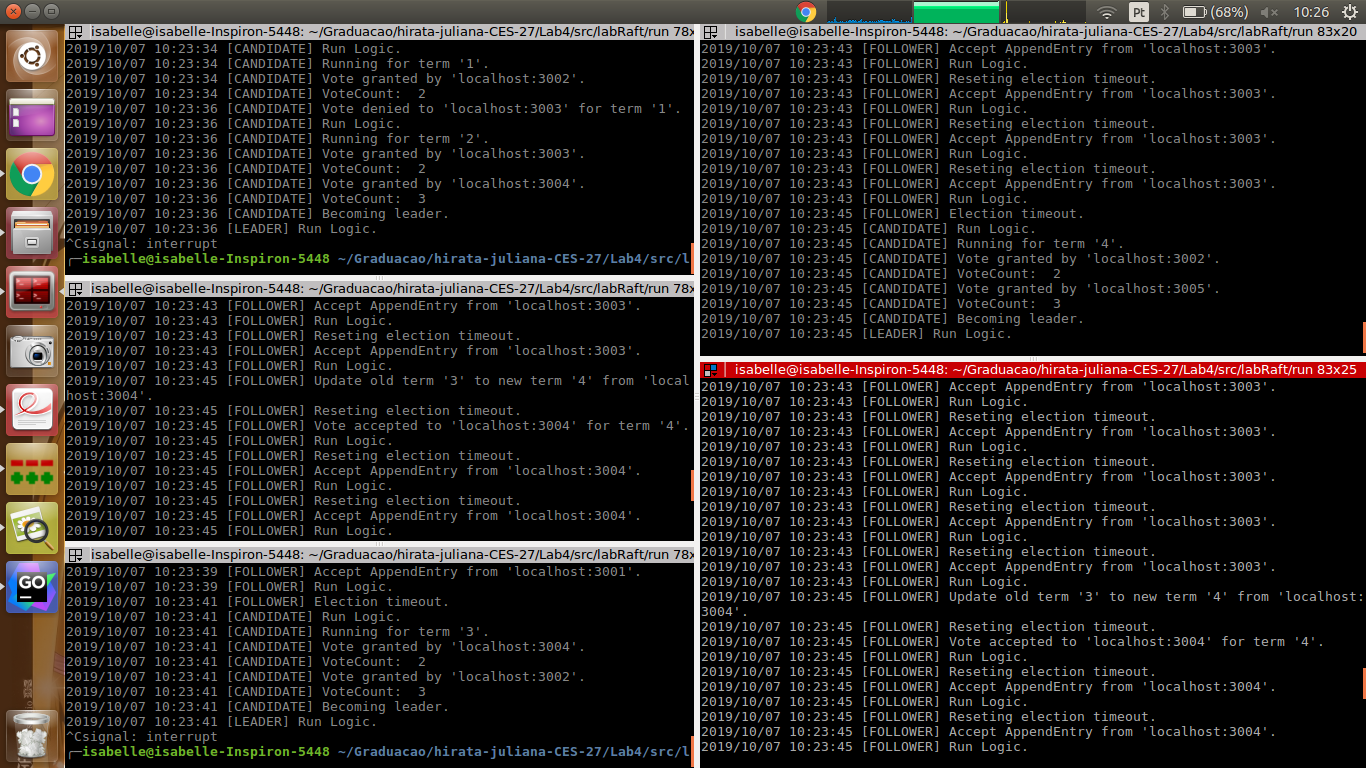
\includegraphics[scale=0.4]{imagens/2_falhas.png}}
\caption{Funcionamento após a falha no próximo \textit{leader}.}.
\label{2_falhas}
\end{figure}

Na Figura \ref{3_falhas}, foi apresentado uma captura de tela de um funcionamento com falha de três instâncias, também sem retomadas dos servidores falhos. Note que o sistema não consegue mais decidir por um novo \textit{leader}.

\begin{itemize}
\item Server 1 (\textit{leader}) falha
\item Server 5 vida \textit{candidate}
\item Server 5 recebe voto de 3 e 4 (e vira \textit{leader}), e de 2
\item Server 5 (\textit{leader}) falha
\item Server 3 vira \textit{candidate}
\item Server 3 recebe voto de 4 e 2 (e vira \textit{leader})
\item Server 3 (\textit{leader}) falha
\item Server 4 vira \textit{candidate}
\item Server 4 recebe voto de 2
\item Server 4 não virará \textit{leader}, pois só teve 2 votos (o de 2 e o dele mesmo)
\item Server 2 continua indefinidamente como \textit{follower} (sem nenhum \textit{leader})
\end{itemize}

\begin{figure}[H]
\centering
\centerline{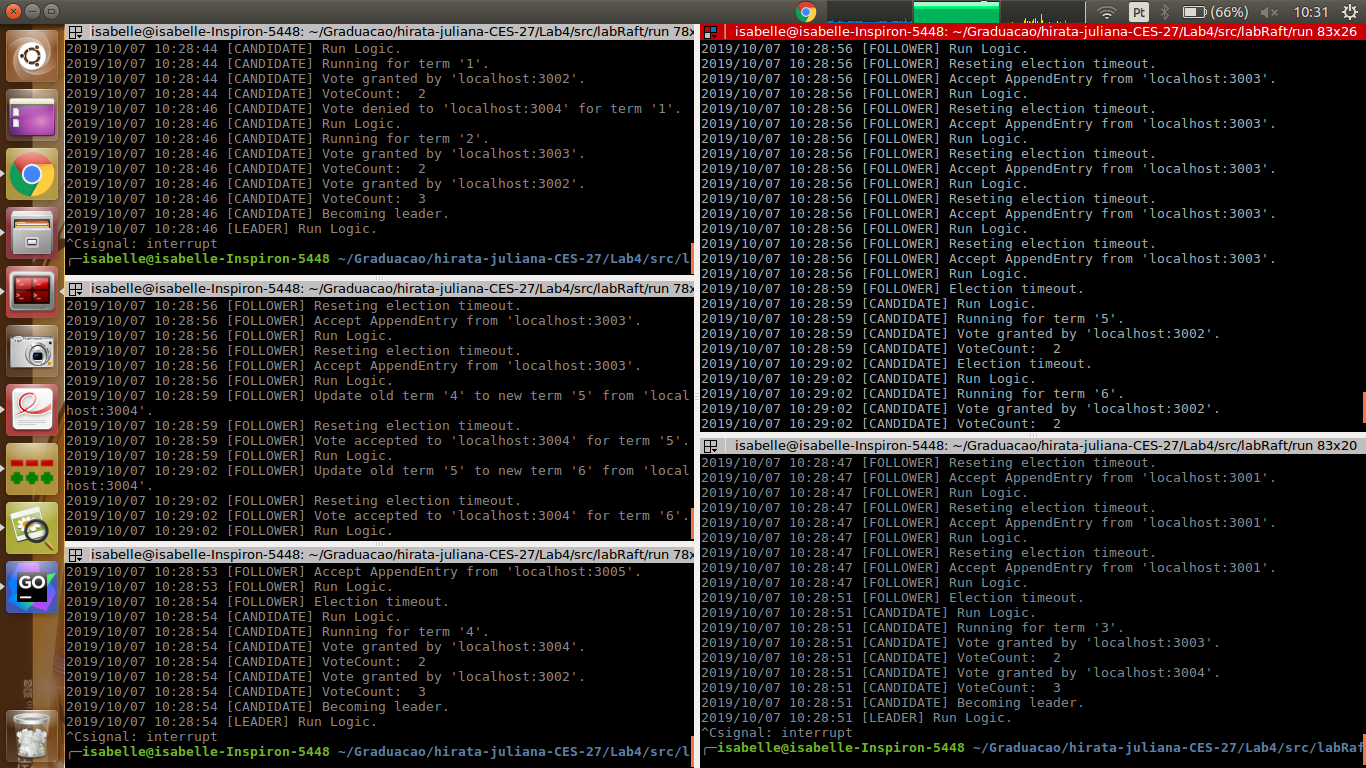
\includegraphics[scale=0.4]{imagens/3_falhas.png}}
\caption{Funcionamento após a falha no terceiro \textit{leader}. Note que o sistema não consegue mais decidir por um novo \textit{leader}.}.
\label{3_falhas}
\end{figure}

\end{document}
